\documentclass[11pt,pdftex,a4paper]{scrartcl}
\usepackage[top=2.5cm, bottom=2.5cm, left=3cm, right=3cm]{geometry}
\usepackage[english,ngerman]{babel}
\usepackage{sourceserif}
\usepackage{sourcesans}
\usepackage[utf8]{inputenc}
\usepackage[babel,german=quotes]{csquotes}
\usepackage[T1]{fontenc}
\usepackage{graphicx}
\usepackage[style=geographie_koeln,dashed=false,maxcitenames=2,maxbibnames=99,backend=biber,urldate=short,firstinits=true,uniquename=false,babel=other,uniquelist=false]{biblatex}
\usepackage{caption}
\captionsetup{
	font={small, stretch=1},
	labelfont=bf
}

\linespread{1.5}

%\setkomafont{section}{\normalfont\bfseries}
%\setkomafont{subsection}{\normalfont\bfseries}
%\setkomafont{}{\normalfont\bfseries}

\newcommand{\leadingzero}[1]{\ifnum #1<10 0\the#1\else\the#1\fi}
\newcommand{\datumVonHeute}{\leadingzero{\day}.\leadingzero{\month}.\the\year}

\bibliography{test,BA}

\newcommand{\haThema}{Routingbasierte ÖPNV-Indikatoren im Rheinland}
\newcommand{\haAutor}{Paul Jannis Weiland}
\newcommand{\haAutorAdresse}{Plankgasse 58}
\newcommand{\haAutorPLZ}{50668}
\newcommand{\haAutorOrt}{Köln}
\newcommand{\haDeckblattTextEins}{Abschlussarbeit}
\newcommand{\haDeckblattTextZwei}{Bachelor of Arts Geographie}
\newcommand{\haSchule}{Universität zu Köln}
\newcommand{\haSchuleAdresse}{Albertus-Magnus-Platz}
\newcommand{\haSchulePLZ}{50923}
\newcommand{\haSchuleOrt}{Köln}
\newcommand{\haGutachter}{Dr. Christian  Willmes}
\newcommand{\haGutachterText}{}

\title{\haThema}
\author{\haAutor}
\date{\today}

\begin{document}
	
	% DECKBLATT
	\begin{titlepage}
		Universität zu Köln\\
		Geographisches Institut
		\begin{center}
			\vspace{1.5cm}
			{\scshape\large \haDeckblattTextEins \par}
			\vspace{1cm}
			{\scshape\large zum Thema\par}
			\vspace{1.5cm}
			{\LARGE\bfseries \haThema \par}
			\vfill
			{Erstellt von:\\ {\bfseries \haAutor}\\ \haAutorAdresse\\ \haAutorPLZ~\haAutorOrt \par}
			\vspace{1cm}
			{\haDeckblattTextZwei \\ \haSchule \\ \haSchuleAdresse \\ \haSchulePLZ~\haSchuleOrt \par}
			\vspace{1cm}
			Gutachter:\\ {\bfseries \haGutachter}\\ \haGutachterText
			\vfill
		\end{center}
		{\haAutorOrt,~\datumVonHeute\par}
	\end{titlepage}
	\thispagestyle{empty}
	\newpage
	
	% INHALTSVERZEICHNIS
	\tableofcontents
	\thispagestyle{empty}
	\newpage
	
	% Seitenzahl auf 1 setzen
	\setcounter{page}{1}
%\begin{document}
\section{Einleitung}
Hier steht normaler Text ohne jede Besonderheit, sozusagen der Fließtext.\\
\texttt{Wie sieht dieser Text aus, er soll eine Art Codeausschnitt darstellen?}
\section{Literatur}
\subsection{Netzwerke}
\subsection{ÖPNV in Deutschland und Nordrhein-Westfalen}
\subsection{Access}
\subsection{Indikatoren}
%evtl Access und Indikatoren in eins.
\section{Methodik}
Im Folgenden soll beschrieben werden, wie 
\subsection{Vorstellung des Untersuchungsgebietes}
Untersucht werden soll das Gebiet des Regierungsbezirks Köln (5.866 – 7.7918°O, 50.323 – 51.251°N), deckungsgleich mit dem Zuständigkeitsbereich des Zweckverbandes go.Rheinland, Aufgabenträger für den SPNV und den Verkehrsverbünden VRS („Verkehrsverbund Rhein-Sieg“) und AVV („Aachener Verkehrsverbund“).
\begin{figure}[h]
	\centering
	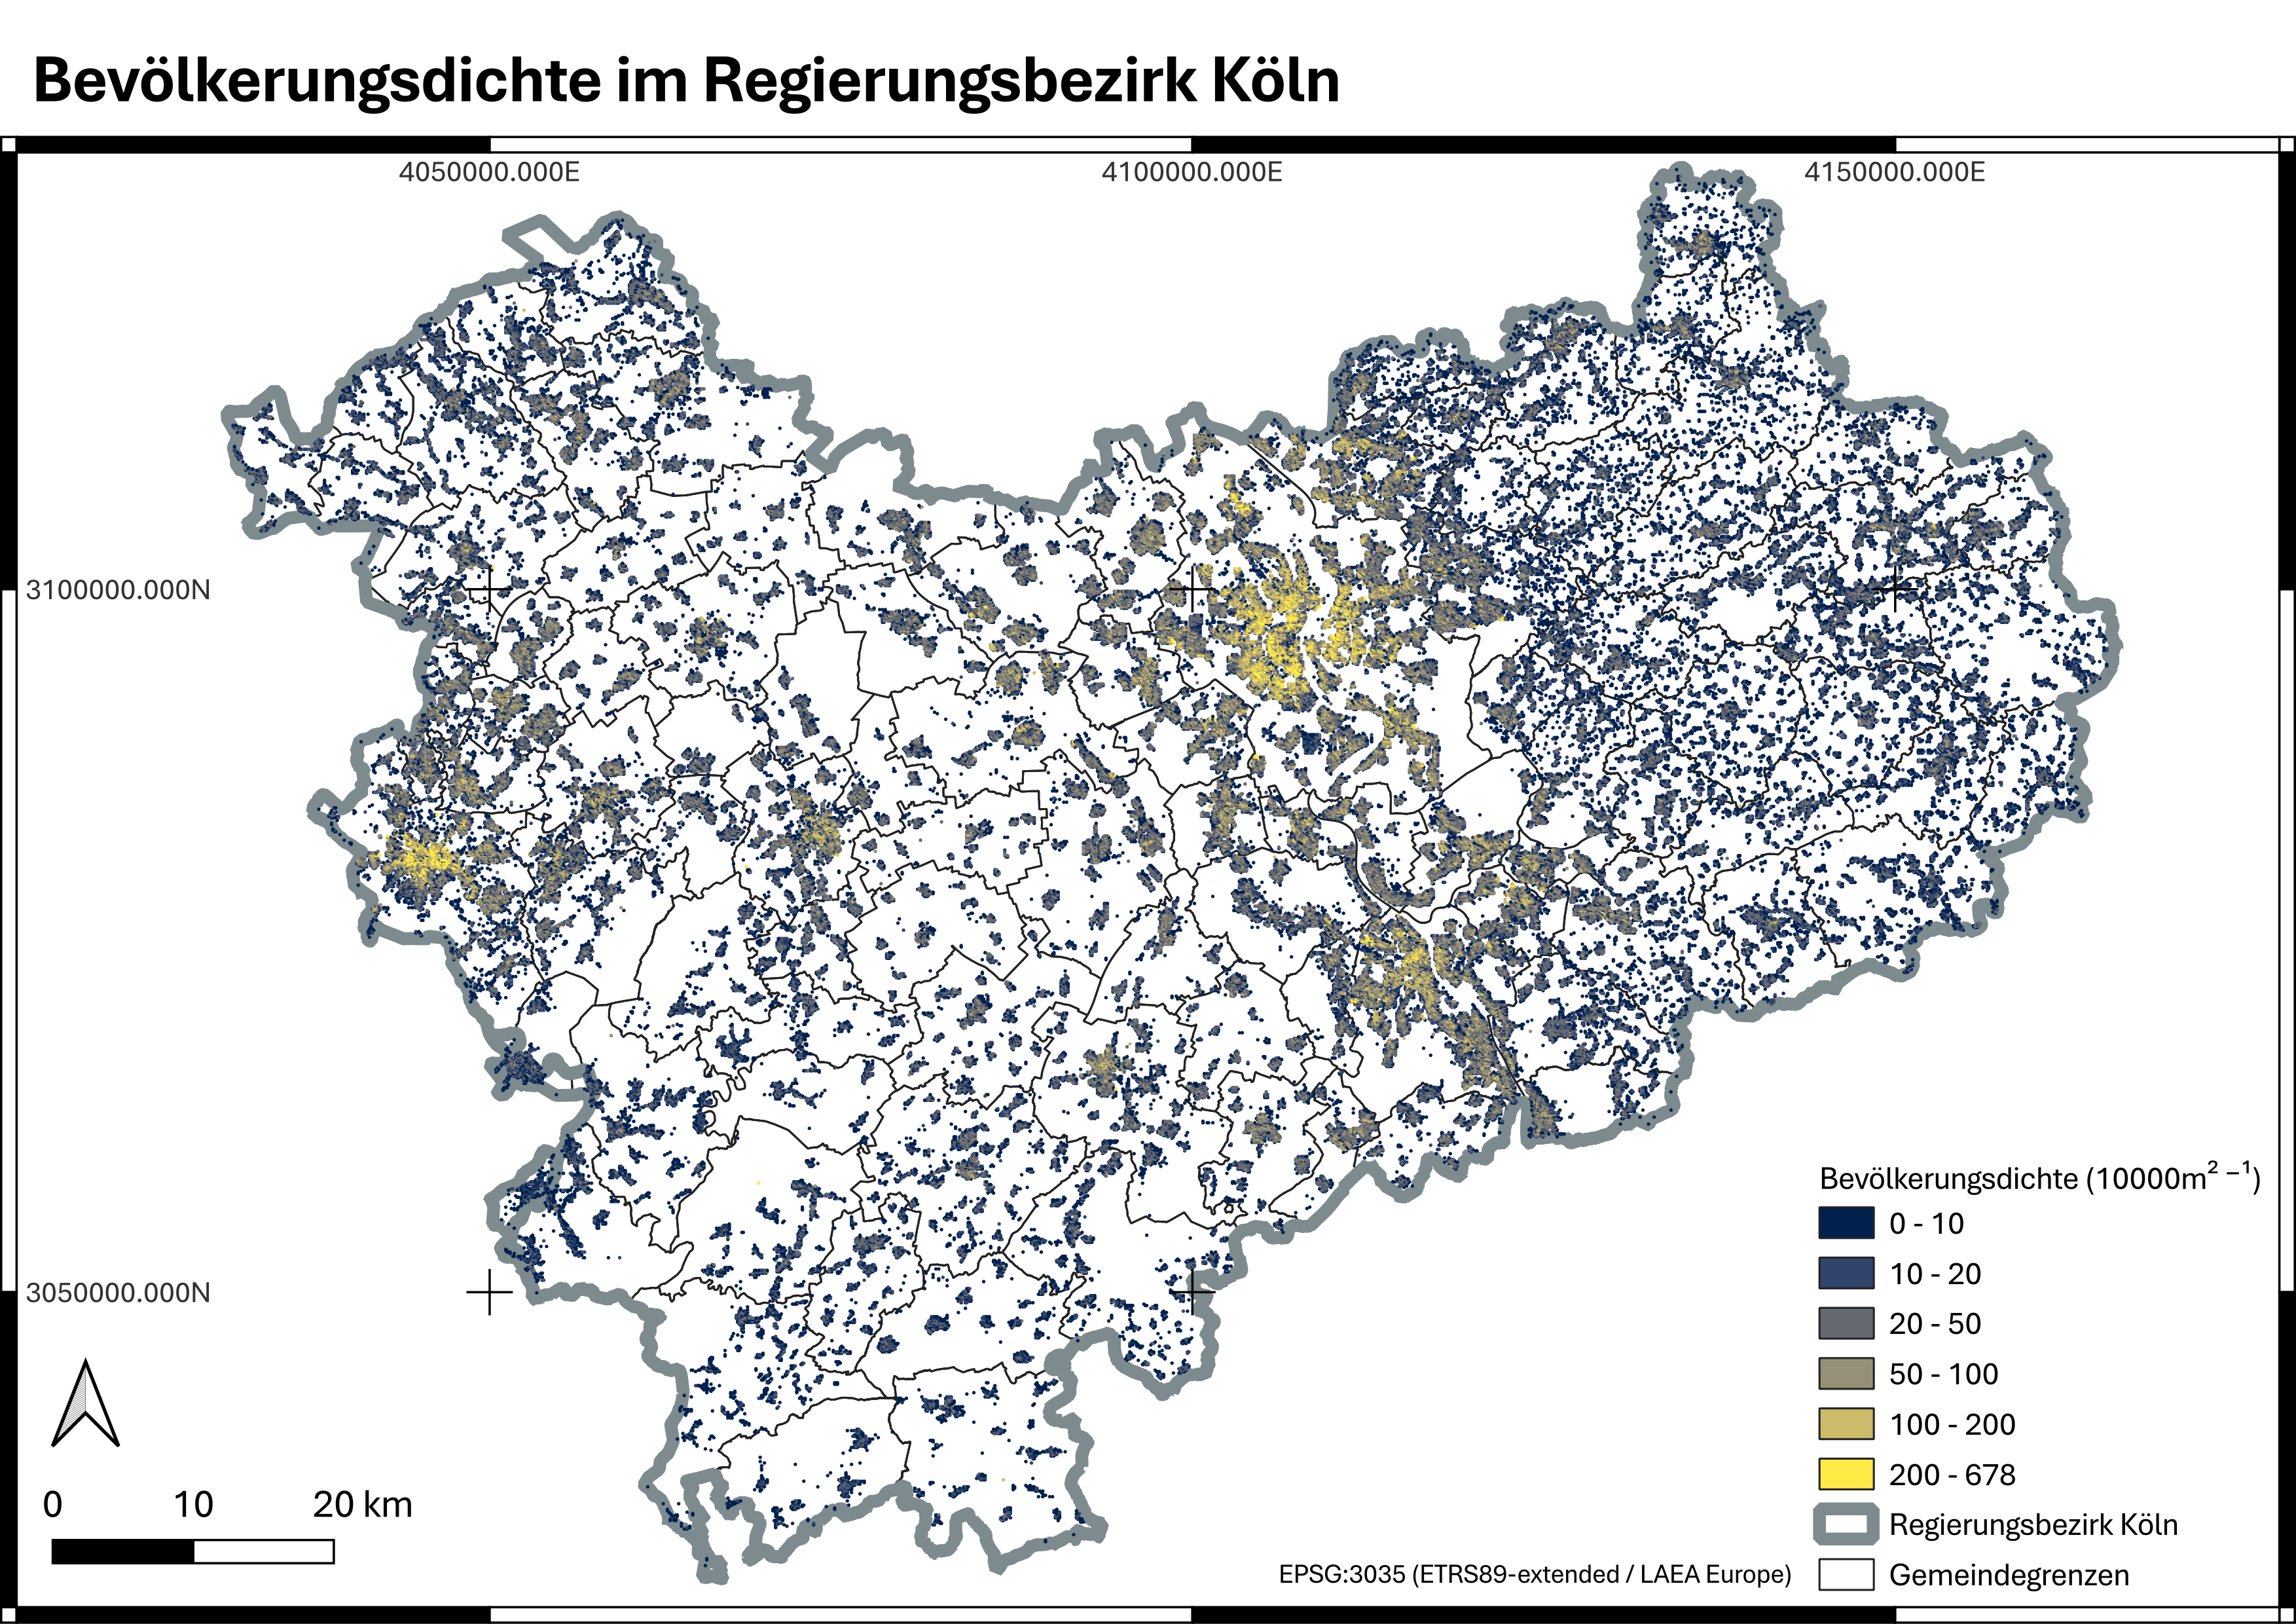
\includegraphics[width=1\linewidth]{figures/Popdensity}
	\caption{Umriss des Untersuchungsgebiets mit Gemeindegrenzen und Bevölkerungsdichte auf Grundlage des Zensus 2022. \parencite{statistischeamterdesbundesundderlanderErgebnisseZensus20222022}}
	\label{fig:popdensity}
\end{figure}
In diesem Gebiet liegt eine heterogene Siedlungsstruktur mit den städtischen Ballungsräumen Köln, Bonn, Aachen und Leverkusen und ländlicheren, weniger dicht besiedelten Räumen vor:  Die Nordeifel im Südwesten und das bergischen Land im Osten. Diese ländlichen Räume unterscheiden sich zusätzlich durch verschiedene Siedlungsanordnungen: Östlich des Rheins (Rheinisch-Bergischer Kreis, Rhein-Sieg-Kreis und Oberbergischer Kreis) liegen (räumlich) kleinere Siedlungen dichter beieinander, westlich (Kreis Euskirchen, Kreis Düren, Rhein-Erft-Kreis, in geringerem Maße Kreis Heinsberg) sind die Siedlungsflächen tendenziell etwas größer und liegen weiter auseinander. Daraus ergeben sich verschiedene Anforderungen an die lokalen Verkehrsnetze und vielfältige Pendlerverflechtungen (Umland-Stadt, Stadt-Umland, Stadt-Stadt). 

Durch den Strukturwandel im rheinischen Braunkohlerevier und die im Investitionsgesetz Kohleregionen verankerten Mittel zur Förderung der Eisenbahn- und eisenbahnanliegenden Infrastruktur (Investitionsgesetz Kohleregionen 2023, §§ 22, 27, Anlage 4) ergibt sich zusätzlicher Handlungs- und Informationsbedarf, der eine Untersuchung des verkehrlichen Status Quo des Gebietes relevant macht. Die verwendeten Methoden sind, aufgrund der deutschlandweit verfügbaren Datenquellen, zwar auf ganz Deutschland anwendbar, werden aufgrund des angestrebten Detailgrades der Auswertung und der resultierenden Notwendigkeit, eventuelle Randbedingungen und Ungenauigkeiten manuell zu prüfen auf das beschriebene Gebiet heruntergebrochen.
\subsection{Datengrundlagen}
\subsubsection{OSM}
\subsubsection{GTFS}
\subsubsection{Zensus}
\subsection{Berechnung der Indikatoren}
\subsubsection{Erschließungsqualität}
Für die Berechnung der Erschließungsqualität nach den Indikatoren des Bundesministeriums für Digitales und Verkehr \parencite[25-27]{bmdvIndikatorenLeichtGemacht2023} sind folgende Elemente notwendig: Eine Auflistung der Haltestellen im Untersuchungsgebiet mit einer Bedienungsqualität auf Grundlage von Tabelle 1 im Steckbrief \parencite[27]{bmdvIndikatorenLeichtGemacht2023}, eine Anzahl an Startpunkten, von denen aus die Gehzeit zu den umliegenden Haltestellen berechnet wird, und ein routingfähiges Fußwegenetz des Untersuchungsgebietes. Im folgenden soll beschrieben werden, wie diese Daten jeweils bereitgestellt bzw. errechnet werden.
%Die Bedienungsqualität einer Haltestelle ergibt sich für diesen Zweck aus der Kombination der Anzahl der Abfahrten pro Stunde, gemittelt über fünf Wochentage, und dem höchstrangigen Verkehrsmittel an der Haltestelle in drei Kategorien (Bus, Stadt-, Straßen-, U-Bahn oder regionaler SPNV).
\paragraph{Fahrplandaten}

Als Informationsquelle für die Abfahrten dient der deutschlandweite GTFS-Feed des DELFI e.V. \parencite{delfie.v.DeutschlandweiteSollFahrplandatenGTFS2026}, der wöchentlich aktualisiert wird. Dieser Feed wird zunächst mit der Funktion \texttt{filter\_feed\_by\_area()} aus der Bibliothek  \texttt{tidytransit} \parencite{polettiTidytransitReadValidate2025} auf das Untersuchungsgebiet zugeschnitten.  Dabei wird ein Puffer von fünf Kilometern um das Gebiet angesetzt, um Grenzfälle zu vermindern. Der deutschlandweite Feed nutzt die optionale Tabelle \texttt{transfers.txt}. Diese ermöglicht es, auf Grundlage von Entfernungen berechnete Umstiegszeiten zu überschreiben um beispielsweise kürzere oder längere Umstiege zu verzeichnen Außerdem können „in-seat-transfers“, bei denen das gleiche Fahrzeug als anderer trip weiterfährt (d.h. der Umstieg ist möglich, obwohl die Ankunft und Abfahrt sehr nah beeinander liegen), oder Kupplungen und Flügelungen abgebildet werden \parencite{GoogleTransit2026}. Außerdem verwendet er das optionale Feld \texttt{parent\_station} in der \texttt{stops.txt}. Die Halte sind nicht als einzelner Punkt repräsentiert, sondern als einzelne Bahnsteige/Masten/Einstiegsorte, die unter einer \texttt{parent\_station} zusammengefasst sind. \texttt{filter\_feed\_by\_area()} berücksichtigt diese optionalen Werte nicht. Trips, die zum Teil außerhalb des gewählten Bereiches liegen, werden mit ihren \texttt{stops} beibehalten, nicht aber die zugehörige \texttt{parent\_station} (d.h. beispielsweise ein Gleis eines Bahnhofs ist im gefilterten Feed enthalten, nicht aber der Bahnhof selbst). Ebenso verhält es sich mit Routen, die als \texttt{transfer} einer Route im Bereich angegeben sind, aber außerhalb des Bereichs liegen. Das führt zu Validierungsfehlern bei der Verarbeitung des Feeds, weshalb diese Stops und Routen nach dem Filtern wieder hinzugefügt werden. (\texttt{de\_gtfs\_cleaning.R}) Es ist zu prüfen, welche Ergebnisunterschiede sich aus der Aggregierung der Halte an den einzelnen stops unter dem Standort der entsprechenden \texttt{parent\_station} ergeben. Tendenziell ergibt sich eine bessere Bedienungsqualität, allerdings sind liegen die stops einzelner \texttt{parent\_stations} teils weit auseinander, weswegen sich möglicherweise eine unrealistische Verschiebung der Gehzeiten ergeben könnte. Besonders an größeren SPNV-Stationen, bei denen einzelne SPNV-Gleise und Busbahnhöfe unter einer \texttt{parent\_station} zusammengefasst werden, besteht dieses Problem. Die Bedienungsqualität dieser Stationen wird bei Aggregierung tendeziell überbewertet, allgemein ist aber insbesondere bei Bushaltestellen die Aggregierung sinnvoll. Bei (Haupt-) Bahnhöfen mit weit entfernten Bushaltestellen ist eine Einzelprüfung/Trennung denkbar.

Der Indikatorensteckbrief des BMDV setzt für die Berechnung der Bedienungsqualität den Wert der durchschnittlichen Abfahrten pro Stunde zwischen 8 und 18 Uhr an einem „Normalwerktag außerhalb der Ferien“, aggregiert über alle Wochentage hinweg an. Tidytransit erstellt beim Einlesen des Feeds eine Tabelle dates\_services, in der auf Grundlage der calendar.txt und der calendar\_dates.txt des Feeds verzeichnet ist, an welchem Tag welcher Service aktiv ist. Diese wird so gefiltert, das nur Wochentage, die kein Feiertag sind, übrig bleiben, anhand der service\_id mit den trips verschnitten, so dass nur jene Fahrten übrig bleiben, die an diesen Tagen verkehren. Zusätzlich werden die route\_types aus der routes.txt angehängt, damit Fernverkehre herausgefiltert werden können.  Anhand dieses Datensatzes werden die stop\_times gefiltert und Halte vor 08:00 und nach 18:00 entfernt. Anschließend werden die stops mit der globalen Haltestellen-ID, die im zentralen Haltestellenverzeichnis referenziert ist, angehängt. Um schließlich die mittleren Abfahrten pro Stunde zu erhalten, wird nach Haltestellen-ID gruppiert, die Halte gezählt und durch die Anzahl der Tage und Stunden geteilt, das höchstrangige Verkehrsmittel anhand der route\_types identifiziert und eine Bedienungsqualität entsprechend der Tabelle zugewiesen.

Schwierigkeiten ergeben sich aus der Formulierung in der Publikation des BMDV. Auf Seite 25 ist von „einem Normalwerktag außerhalb der Ferien“ die Rede, in der Tabelle wird ein Durchschnitt über fünf Wochentage betrachtet. Da es keinen „Soll“-GTFS-Feed gibt, der einen Idealzustand des Netzes ohne Ausfälle, Baustellen, Sonderfahrten bzw. Ausfällen aufgrund von Großveranstaltungen  gibt, stellt sich die Frage, wie eine repräsentative Abbildung der Bedienungsqualitäten extrahiert werden kann.

r5r stellt mit check\_transit\_availability eine Möglichkeit zur Analyse der Variabilität des Feeds zur Verfügung. Es wird auf Grundlage des Netzwerkgraphen, der mit build\_network erstellt wurde, extrahiert, wie viele der services aus dem GTFS-Feed an welchen Daten aktiv sind. Der Feed des DELFI e.V. vom 30.03.2026 im Zuschnitt auf das Gebiet des Regierungsbezirks Köln zeigt eine Variabilität von 10,12\% (min = 20,73\% am 15.03 (Sonntag), max = 30,86\% am 24.04. (Freitag)). Ohne Wochenenden ergibt sich immer noch eine Varianz von 8,31\% mit min = 22,54\% am 19.03. (Donnerstag). 
% latex table generated in R 4.5.2 by xtable 1.8-8 package
% Mon May 25 18:34:59 2026
\begin{table}[ht]
	\centering
	\begin{tabular}{rlrrrr}
		\hline
		& weekday & avg\_pct & avg\_services & sd\_services & variance\_services \\ 
		\hline
		1 & Samstag & 0.21 & 1035.21 & 115.34 & 13304.23 \\ 
		2 & Sonntag & 0.18 & 931.03 & 102.06 & 10417.26 \\ 
		3 & Montag & 0.22 & 1094.62 & 111.33 & 12395.21 \\ 
		4 & Dienstag & 0.22 & 1095.44 & 114.86 & 13193.54 \\ 
		5 & Mittwoch & 0.22 & 1098.41 & 119.74 & 14337.35 \\ 
		6 & Donnerstag & 0.22 & 1089.28 & 115.96 & 13447.69 \\ 
		7 & Freitag & 0.23 & 1151.50 & 125.36 & 15715.35 \\ 
		\hline
	\end{tabular}
\end{table}
\begin{figure}
	\centering
	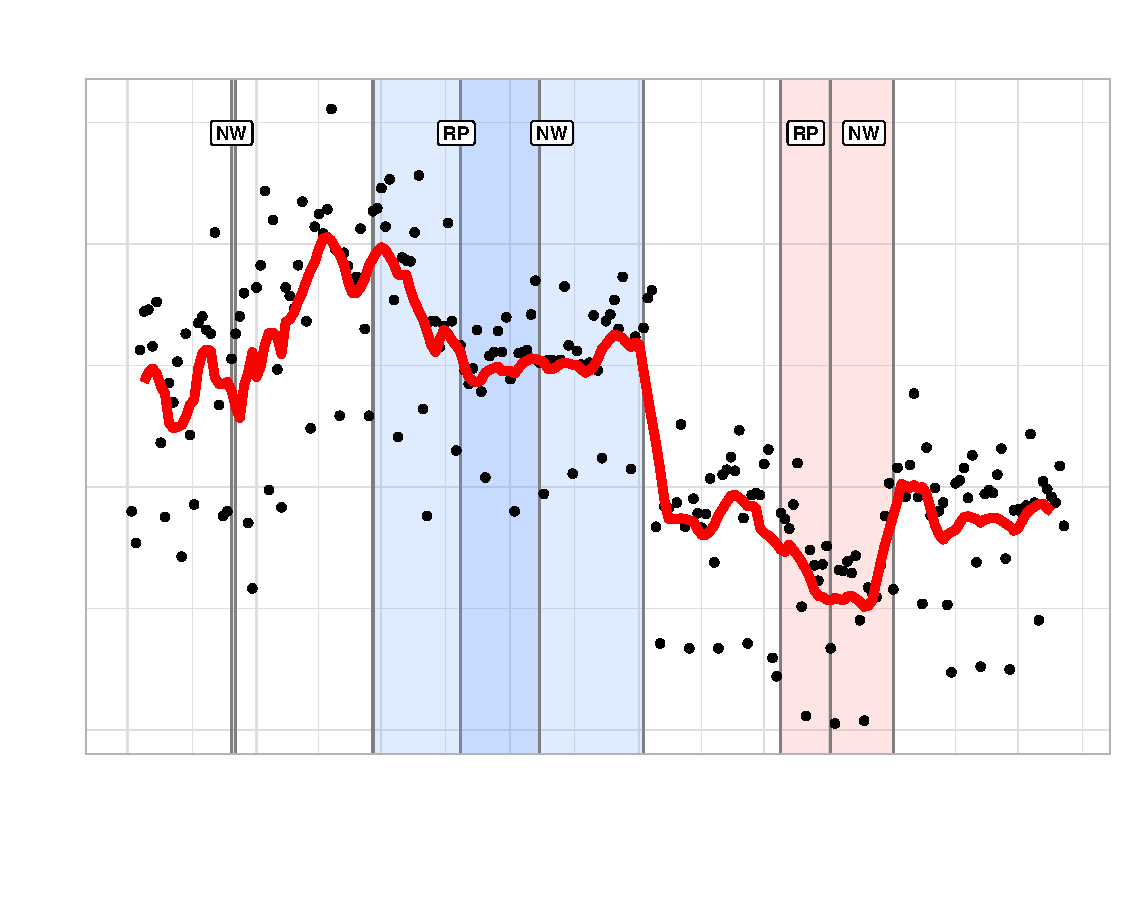
\includegraphics[width=1\linewidth]{figures/active_services_year_rollavg_2026-05-18}
	\caption{Variabilität des Anteils der aktiven services im GTFS-Datensatz.}
	\label{fig:activeservicesyearrollavg2026-05-18}
\end{figure}

Um die Varianz der Fahrplandaten über mehrere Tage und Wochen darzustellen soll die Bedienungsqualität für die Abfahrten jedes einzelnen verfügbaren Tag des Feeds berechnet werden. Diese Daten werden mit einer (statischen) Reisezeitmatrix (Zensusgitter Haltestellen) verrechnet, pro Tag die jeweils beste Möglichkeit ermittelt und die Varianz als gesamte Distanz (Häufige Wechsel zwischen bspw. Erschließungsqualität A und Erschließungsqualität B ergeben einen hohen Wert genauso wie wenige Wechsel zwischen bspw. A und F) und als Spanne (maximale Differenz in der Erschließungsqualität) berechnet werden. 


\section{Ergebnisse}
\subsection{Indikatoren}
\subsection{Weiße Flecken} %Arbeitstitel
\section{Diskussion}
\section{Fazit}
Monographiezitat im Fließtext: \textcite[1]{Buchautor2000}

Monographiezitat: \parencite[1]{Buchautor2000}

Schriftenreihe: \parencite[22]{Schriftenreihler2000}

Beitrag aus Sammelwerk mit zwei Autoren: \parencite[12]{Sammler2000}

Englisher Beitrag aus Sammelwerk mit zwei Autoren: \parencite[12]{Collector2000}

Zeitschriftenartikel mit 4 Autoren: \parencite[11]{Zeitschriftler2000}

Konferenzbeitrag: \parencite[200]{Konferenzler2000}

Englischer Konferenzbeitrag: \parencite[200]{ConferenceGuy2000}

Doktorarbeit: \parencite[12]{Doktor2000}

Internetquelle, nicht von Person, sondern von Organisation: \parencite{Internetorganisation2000}

Internetquelle mit DOI: \parencite{Onlinedoiautor2000}

Zeitungsartikel: \parencite{Kolumna2000}

Karte: \parencite{Kartenorganisation2000}

\printbibliography
\end{document}
